\documentclass{beamer}
\usepackage{tikz}
\usetheme{Madrid}
\usepackage{ctex}
\usecolortheme{default}
\usepackage{verbatim}
\title[2022.12.12日汇报] %optional
{2022.12.12汇报}
%\subtitle{Demonstrating the Berkeley theme}
\author[周添文] % (optional)
{周添文\inst{} }

\institute[] % (optional)
{
  \inst{}%
  数学科学学院\\
  北京师范大学\\
 % \and
  %\inst{2}%
%  Faculty of Chemistry\\
%  Very Famous University
}

\date[2022.12.12] % (optional)
%{Very Large Conference, April 2021}

% Use a simple TikZ graphic to show where the logo is positioned

%\node[draw,color=white] at (0,0) {LOGO HERE};


%End of title page configuration block
%------------------------------------------------------------
%The next block of commands puts the table of contents at the 
%beginning of each section and highlights the current section:

\AtBeginSection[]
{
  \begin{frame}
    \frametitle{Table of Contents}
    \tableofcontents[currentsection]
  \end{frame}
}
%------------------------------------------------------------
\begin{document}
\frame{\titlepage}
%\logo{\includegraphics[]{bnu.png}}
%---------------------------------------------------------
%Highlighting text
\begin{frame}
\frametitle{Radon变换}
在上周的文章中,作者对方程
\begin{equation}
\hat{\widetilde{F}}_k(\textbf{x}_{global})=\widetilde{G}_k(\textbf{x}_{global})-I(\textbf{x}_{global})
\end{equation}
得到的$\hat{\widetilde{F}}_k(\textbf{x}_{global})$,关于每一帧$k$进行Radon变换,下面我们探究Radon变换的方法和意义。\pause

整体上来说,Radon变换是用于进行直线探测的工具。具体而言,其本质是将原来的函数做了一个空间转换,即,将原来的$XY$平面内的点映射到$AB$平面上,那么原来在$XY$平面上的一条直线的所有的点在$AB$平面上都位于同一点。记录$AB$平面上的点的积累厚度,便可知XY平面上的\textbf{线的存在性}。\pause 
\end{frame}
\begin{frame} 
\frametitle{Radon变换的操作}
首先,对于平面中的任意一条直线,我们可以用如下的$\rho, \theta$表示法进行表示:
\begin{equation}
L(\rho,\theta)=\{(x,y):xcos\theta +ysin\theta=\rho\}
\end{equation}\pause

其几何意义见下图:
\begin{figure}[!h]
\centering
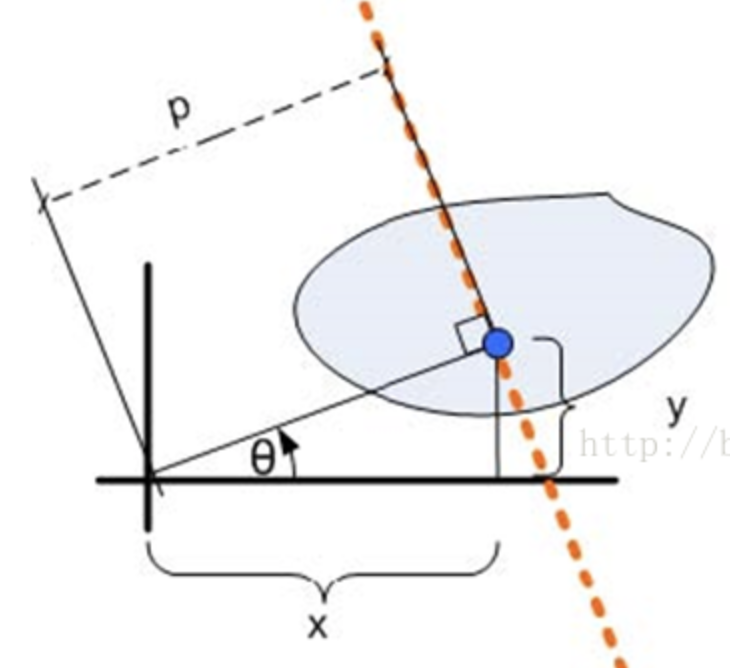
\includegraphics[height=3cm,width=4cm]{20221209.png}
\caption{直线参数式的几何意义}
\end{figure}
\end{frame}
\begin{frame}
\frametitle{Radon变换的操作}
取$f(x,y)$为图像的灰度(或辐照度)函数,则由曲线积分的物理意义
\begin{equation}
\int_Lf(x,y)ds
\end{equation}
表示沿图像上某一条直线$L$的灰度之和。对于不同的直线$L$,这一积分的值越大,代表这一直线上的灰度越大,也就意味着在原始图像上,此处\textbf{更有可能是一条直线}。
\end{frame}
\begin{frame}
\frametitle{Dirac函数及其性质}
下面,我们来看如何计算函数的Radon变换值。首先,我们引入Dirac函数\pause

我们知道,Dirac函数是一个广义函数,其定义如下:
\begin{equation}
\delta(x)=0,(x\neq0)
\end{equation}
\begin{equation}
\int^{\infty}_{-\infty}\delta(x)dx=1
\end{equation}\pause

下面,我们给出Dirac函数的重要性质:
\begin{theorem}
若$\phi(x)$为连续函数,且$\phi(x)$仅有一阶零点$x_k,k=1,2,...$,则:
\begin{equation}
\delta[\phi(x)]=\Sigma^N_{k=1}\frac{\delta(x-x_k)}{|\phi'(x_k)|}
\end{equation}
\end{theorem}\pause
\end{frame}
\begin{frame}
\frametitle{Dirac函数及其性质}
因此,我们有如下公式:
\begin{equation}
\int^{\infty}_{-\infty}g(x)\delta(f(x))dx=\Sigma^N_{k=1}\frac{g(x_i)}{|f'(x_i)|}
\end{equation}
\end{frame}
\begin{frame}
\frametitle{用Dirac函数计算曲线积分}
我们知道,曲线积分的计算方法如下:
\begin{equation}
\int_Lf(\textbf{x})ds=\int^{\infty}_{-\infty}f(x,y(s))\sqrt{1+[y'(x)]^2}dx
\end{equation}\pause
因此,Radon变换可以改写为:
\begin{equation}
\int_Lf(x,y)ds=\int^{\infty}_{-\infty}\int^{\infty}_{-\infty}f(x,y)\delta(xcos\theta+ysin\theta-\rho)dxdy
\end{equation}
\end{frame}
\begin{frame}
\frametitle{Radon变换图}

由此可见,平面上的一条直线$L(\rho,\theta)$唯一对应着一个积分值,对于不同的角度$\theta$而言,其对应着一族直线$L$。因此,各个角度下的不同直线的Radon变换值,构成了一幅\textbf{Radon变换图}。
\begin{figure}[!h]
\centering
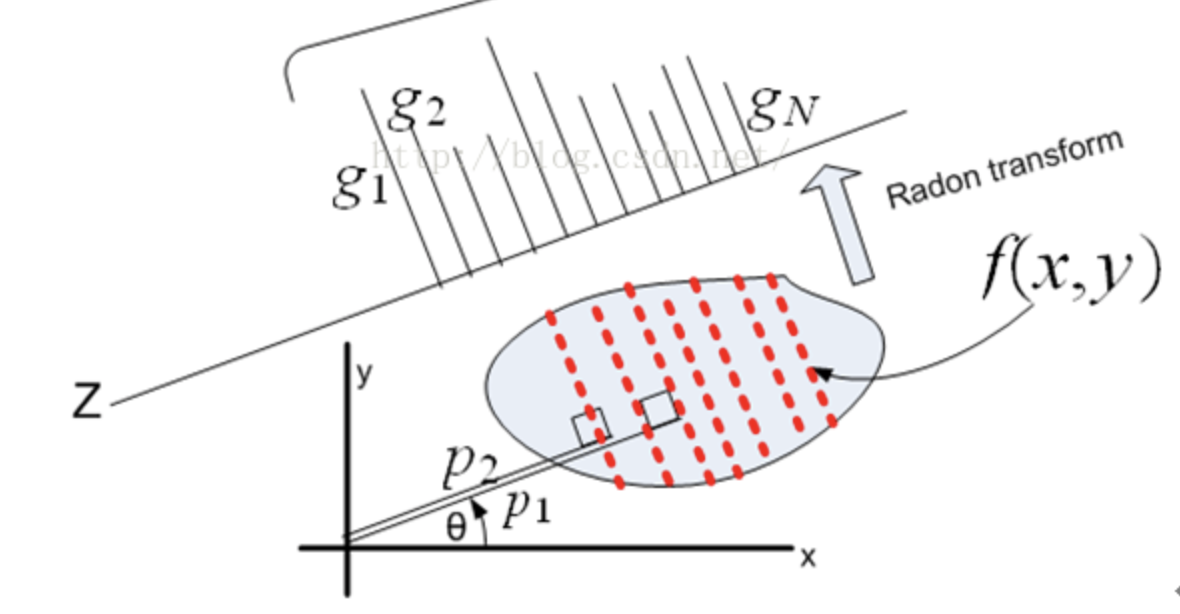
\includegraphics[height=5cm,width=9cm]{2022120901.png}
\caption{Radon变换}
\end{figure}
\end{frame}
\begin{frame}
\frametitle{文章中的操作}
现在,我们回顾文章中的操作,其对耀斑估计的辐照度函数
\begin{equation}
\hat{\widetilde{F}}_k(\textbf{x}_{global})
\end{equation}\pause

进行Radon变换,实际上就是求耀斑图像中的直线对应的线积分值,其形状约接近直线,Radon变换的值也会越大。

而Radon变换图中某一点应的点的亮度则反映了直线$L(\rho,\theta)$对应的积分值大小,积分值越大,该点的亮度也就越大,说明该点对应的直线$L(\rho,\theta)$更有可能是原图像中的一条直线。
\end{frame}
\begin{frame}
\frametitle{耀斑大小的确定}
原文中并未提及如何确定直线附近耀斑的大小,其仅仅说在直线$l_k^{flare}$附近的一个条带(band)上进行操作,但并没有说如何确定条带的带宽。
\end{frame}
\begin{frame}
\frametitle{图像配准的方法}
关于图像配准(对齐)的方法,原文同样没有说明用的是哪种对其方法,但通过学习,我发现目前有许多成熟的图像对齐方法,也有可以直接操作的程序或软件可用。\pause

其基本的目的是将一个场景的不同图片转换到相同的坐标系中。而其原则是将空间中同一位置的点一一对应起来,进行信息融合。\pause

其主要的步骤为:
\begin{itemize}
\item 特征检测
\item 特征匹配
\item 转换模型估计
\item 图像重采样、图像转换
\end{itemize}
\end{frame}
\begin{frame}
\frametitle{图像配准的方法}
目前已有的成熟方法如下:
\begin{figure}[!h]
\centering
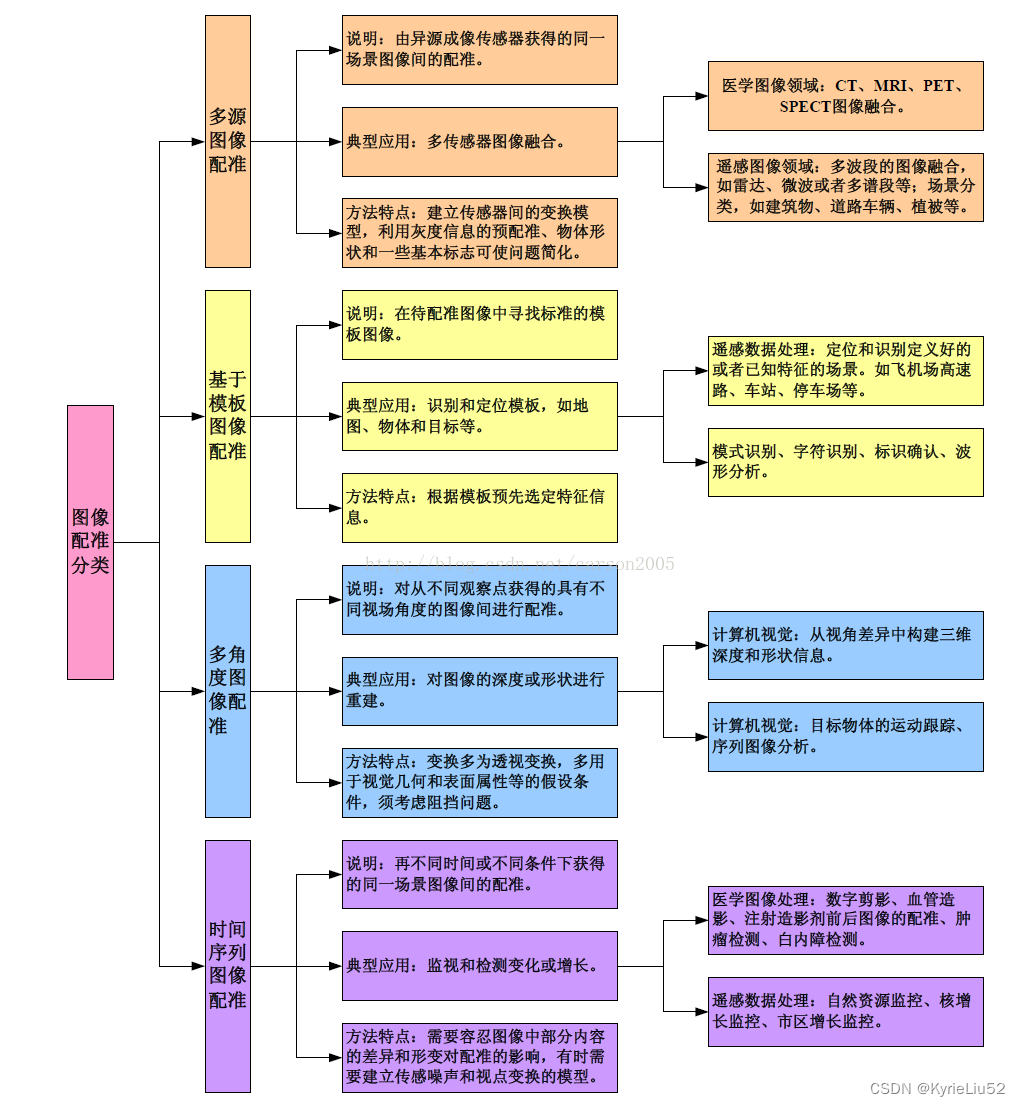
\includegraphics[height=6cm,width=6cm]{2022120902.png}
\caption{图像配准方法}
\end{figure}
\end{frame}
\end{document}